\section{Testing e analisi dei risultati}

%=======================================================================

\begin{frame}{Sotto-famiglie di ASCON}
    \begin{columns}

    \begin{column}{0.28\textwidth}

    \begin{block}{Hash}
        \begin{center}
            Algoritmi hash e XOF
        \end{center}
    \end{block}

    \end{column}
    
    \begin{column}{0.38\textwidth}

    \begin{block}{AEAD}
        \begin{center}
            Algoritmi di cifratura autenticata
        \end{center}
    \end{block}

    \end{column}

    \begin{column}{0.28\textwidth}

    \begin{block}{Auth}
        \begin{center}
            Algoritmi MAC e PRF
        \end{center}
    \end{block}

    \end{column}

    \end{columns}

    \vspace{14pt}

    \begin{center}
        Per ogni sotto-famiglia qui citata è stato scelto un algoritmo e analizzato per tempi di esecuzione e spazio utilizzato; i risultati di tale analisi sono riportati in due tipi di grafico
    \end{center}

    \begin{columns}

    \begin{column}{0.5\textwidth}
        \begin{block}{Tempi di esecuzione}
            \begin{center}
                Contiene gruppi di tre colonne che rappresentano, per ogni implementazione, le misurazioni minima, media e massima
            \end{center}
        \end{block}
    \end{column}

    \begin{column}{0.5\textwidth}
        \begin{block}{Spazio utilizzato}
            \begin{center}
                Contiene una sola colonna per ogni implementazione e ognuna indica la dimensione dell'eseguibile
            \end{center}
        \end{block}
    \end{column}
        
    \end{columns}

\end{frame}

%=======================================================================

\begin{frame}{AEAD: ascon128a}

    \begin{center}
        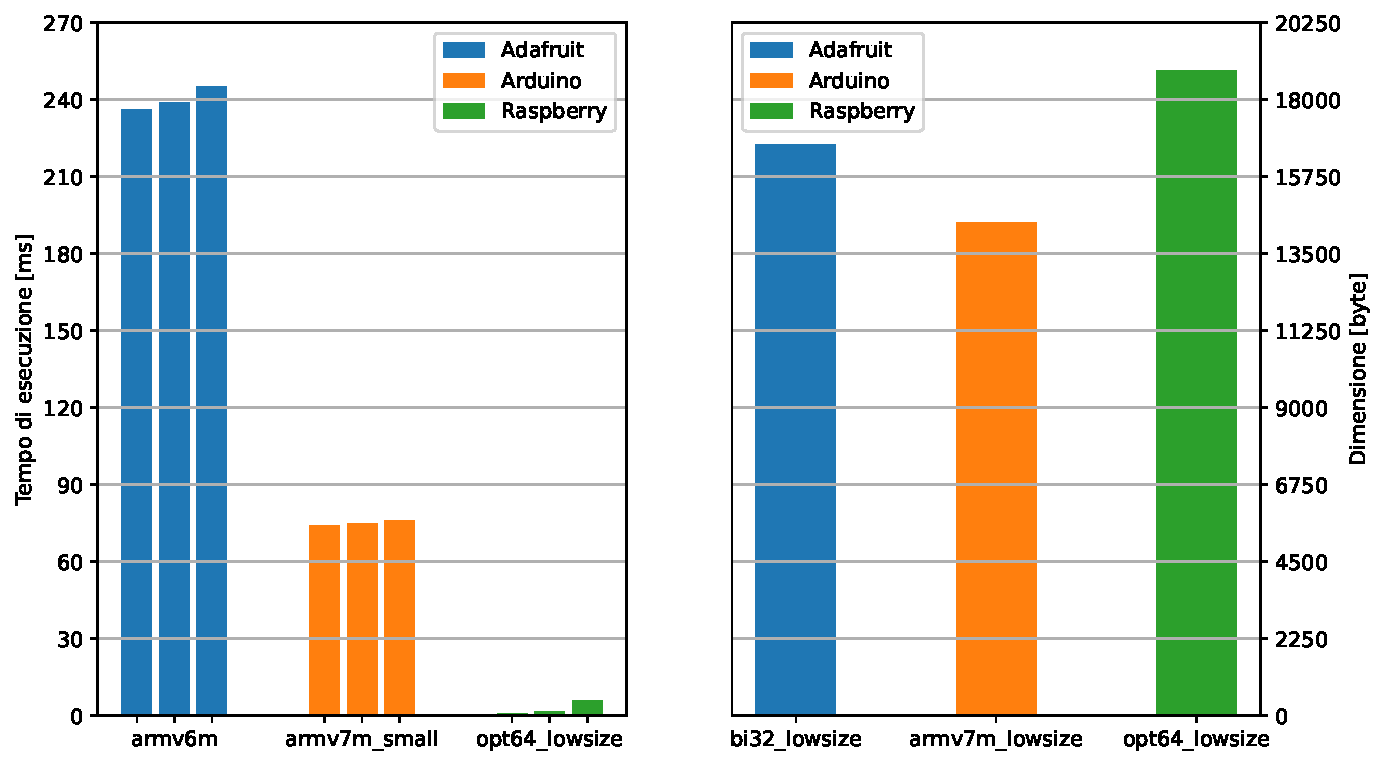
\includegraphics[height=0.40\textwidth]{images/analysis/aead.pdf}
    \end{center}
    
\end{frame}

%=======================================================================

\begin{frame}{Hash: asconhasha}

    \begin{center}
        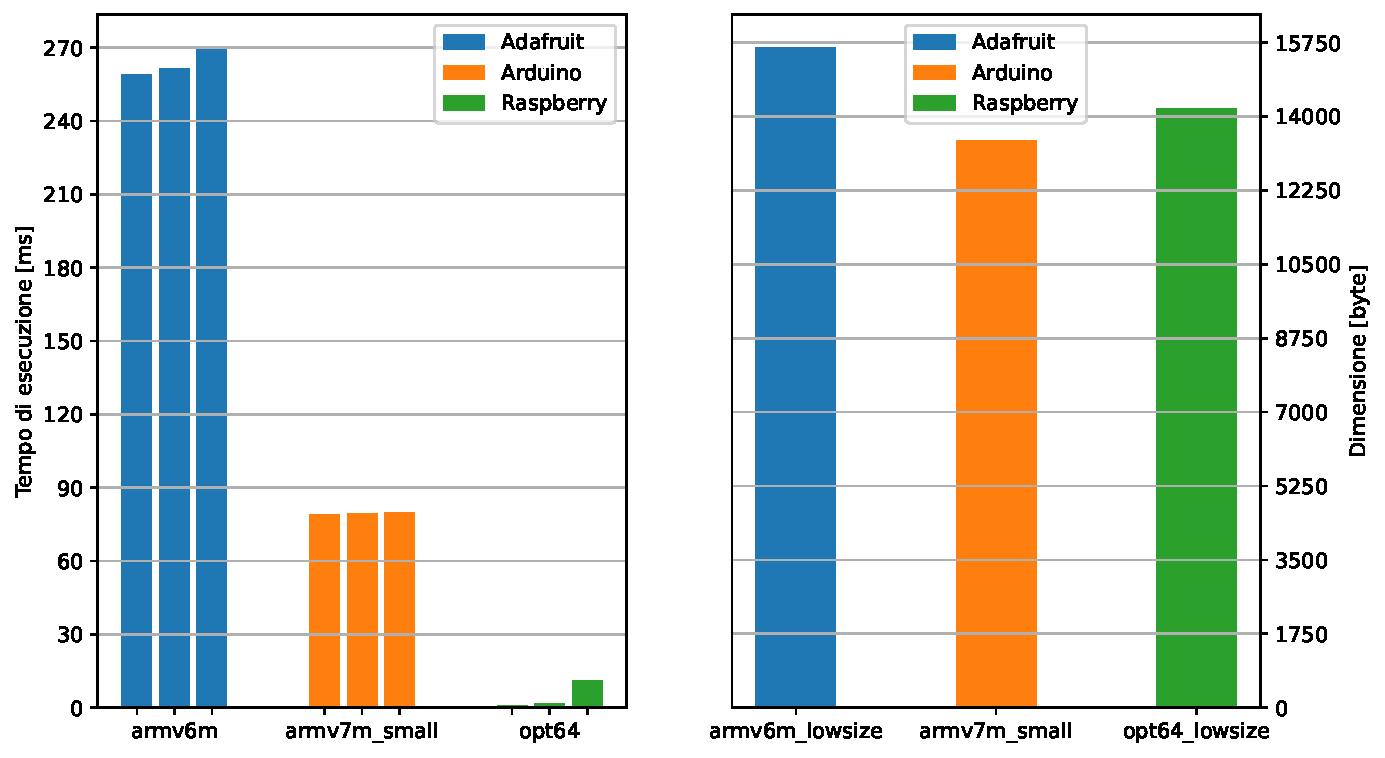
\includegraphics[height=0.40\textwidth]{images/analysis/hash.pdf}
    \end{center}
    
\end{frame}

%=======================================================================

\begin{frame}{Auth: asconmaca}

    \begin{center}
        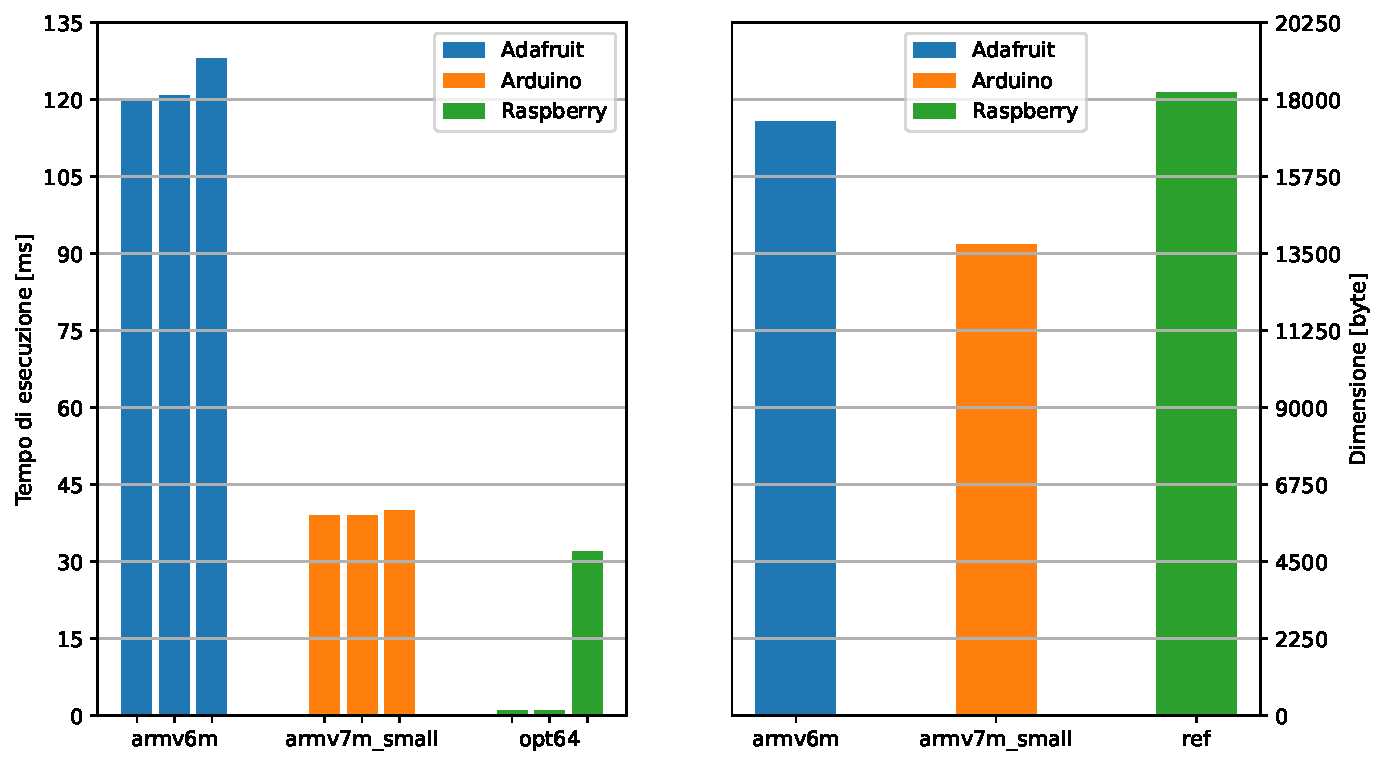
\includegraphics[height=0.40\textwidth]{images/analysis/auth.pdf}
    \end{center}
    
\end{frame}

%=======================================================================

\begin{frame}{Migliori implementazioni per ogni dispositivo}

    \begin{table}
        \centering
        \begin{tblr}{
            cells = {c},
            cell{1}{1} = {r=2}{},
            cell{1}{2} = {c=3}{},
            vlines,
            hline{1,3-6} = {-}{},
            hline{2} = {2-4}{},
        }
            \textbf{Dispositivo} & \textbf{Ottimizzazione proposta} & & \\
            & \textbf{Tempo} & \textbf{Spazio} & \textbf{Ibrida} \\
            \textbf{Adafruit} & \texttt{armv6m} & \texttt{lowsize} & \texttt{armv6m} \\
            \textbf{Arduino} & \texttt{armv7m\_small} & \texttt{armv7m\_small} & \texttt{armv7m\_small} \\
            \textbf{Raspberry} & \texttt{opt64} & \texttt{opt64\_lowsize} & \texttt{opt64}
        \end{tblr}
    \end{table}

\end{frame}
